\documentclass{article}
\usepackage{graphicx, tikz-cd, float, titlepic, booktabs} % Required for inserting images
\usepackage{pgfplots}
\pgfplotsset{compat=1.15}
\usepackage{mathrsfs}
\usetikzlibrary{arrows}
\usepackage{amsmath, amssymb, amsthm, amsfonts, siunitx, physics, gensymb}
\AtBeginDocument{\RenewCommandCopy\qty\SI}
\usepackage[version=4]{mhchem}
\usepackage[most,many,breakable]{tcolorbox}
\usepackage{xcolor, fancyhdr, varwidth}
\usepackage[Glenn]{fncychap}
%Options: Sonny, Lenny, Glenn, Conny, Rejne, Bjarne, Bjornstrup
\usepackage{hyperref, cleveref}
\usepackage{icomma, enumitem} %comma as decimal and continue enumerate with [resume]
\usepackage{plimsoll} %use standard state symbol with \stst
\usepackage[danish]{babel}
%%%%%%%%%%%%%%%%%%%%%%%%%%%%%%
% SELF MADE COLORS
%%%%%%%%%%%%%%%%%%%%%%%%%%%%%%
\definecolor{myg}{RGB}{56, 140, 70}
\definecolor{myb}{RGB}{45, 111, 177}
\definecolor{myr}{RGB}{199, 68, 64}
\definecolor{mytheorembg}{HTML}{F2F2F9}
\definecolor{mytheoremfr}{HTML}{00007B}
\definecolor{mylenmabg}{HTML}{FFFAF8}
\definecolor{mylenmafr}{HTML}{983b0f}
\definecolor{mypropbg}{HTML}{f2fbfc}
\definecolor{mypropfr}{HTML}{191971}
\definecolor{myexamplebg}{HTML}{F2FBF8}
\definecolor{myexamplefr}{HTML}{88D6D1}
\definecolor{myexampleti}{HTML}{2A7F7F}
\definecolor{mydefinitbg}{HTML}{E5E5FF}
\definecolor{mydefinitfr}{HTML}{3F3FA3}
\definecolor{notesgreen}{RGB}{0,162,0}
\definecolor{myp}{RGB}{197, 92, 212}
\definecolor{mygr}{HTML}{2C3338}
\definecolor{myred}{RGB}{127,0,0}
\definecolor{myyellow}{RGB}{169,121,69}
\definecolor{myexercisebg}{HTML}{F2FBF8}
\definecolor{myexercisefg}{HTML}{88D6D1}
%%%%%%%%%%%%%%%%%%%%%%%%%%%%%%%%%%%%%%%%%%%%%%%%%%%%%%%%%%%%%%%%%%%%%%
% Box environments for theorems and problems
%%%%%%%%%%%%%%%%%%%%%%%%%%%%%%%%%%%%%%%%%%%%%%%%%%%%%%%%%%%%%%%%%%%%%
\setlength{\parindent}{1cm}
%================================
% Question BOX
%================================
\makeatletter
\newtcbtheorem{question}{Opgave}{enhanced,
	breakable,
	colback=white,
	colframe=myb!80!black,
	attach boxed title to top left={yshift*=-\tcboxedtitleheight},
	fonttitle=\bfseries,
	title={#2},
	boxed title size=title,
	boxed title style={%
			sharp corners,
			rounded corners=northwest,
			colback=tcbcolframe,
			boxrule=0pt,
		},
	underlay boxed title={%
			\path[fill=tcbcolframe] (title.south west)--(title.south east)
			to[out=0, in=180] ([xshift=5mm]title.east)--
			(title.center-|frame.east)
			[rounded corners=\kvtcb@arc] |-
			(frame.north) -| cycle;
		},
	#1
}{def}
\makeatother
%================================
% DEFINITION BOX
%================================

\newtcbtheorem[]{Definition}{Definition}{enhanced,
	before skip=2mm,after skip=2mm, colback=red!5,colframe=red!80!black,boxrule=0.5mm,
	attach boxed title to top left={xshift=1cm,yshift*=1mm-\tcboxedtitleheight}, varwidth boxed title*=-3cm,
	boxed title style={frame code={
					\path[fill=tcbcolback]
					([yshift=-1mm,xshift=-1mm]frame.north west)
					arc[start angle=0,end angle=180,radius=1mm]
					([yshift=-1mm,xshift=1mm]frame.north east)
					arc[start angle=180,end angle=0,radius=1mm];
					\path[left color=tcbcolback!60!black,right color=tcbcolback!60!black,
						middle color=tcbcolback!80!black]
					([xshift=-2mm]frame.north west) -- ([xshift=2mm]frame.north east)
					[rounded corners=1mm]-- ([xshift=1mm,yshift=-1mm]frame.north east)
					-- (frame.south east) -- (frame.south west)
					-- ([xshift=-1mm,yshift=-1mm]frame.north west)
					[sharp corners]-- cycle;
				},interior engine=empty,
		},
	fonttitle=\bfseries,
	title={#2},#1}{def}
\newtcbtheorem[]{definition}{Definition}{enhanced,
	before skip=2mm,after skip=2mm, colback=red!5,colframe=red!80!black,boxrule=0.5mm,
	attach boxed title to top left={xshift=1cm,yshift*=1mm-\tcboxedtitleheight}, varwidth boxed title*=-3cm,
	boxed title style={frame code={
					\path[fill=tcbcolback]
					([yshift=-1mm,xshift=-1mm]frame.north west)
					arc[start angle=0,end angle=180,radius=1mm]
					([yshift=-1mm,xshift=1mm]frame.north east)
					arc[start angle=180,end angle=0,radius=1mm];
					\path[left color=tcbcolback!60!black,right color=tcbcolback!60!black,
						middle color=tcbcolback!80!black]
					([xshift=-2mm]frame.north west) -- ([xshift=2mm]frame.north east)
					[rounded corners=1mm]-- ([xshift=1mm,yshift=-1mm]frame.north east)
					-- (frame.south east) -- (frame.south west)
					-- ([xshift=-1mm,yshift=-1mm]frame.north west)
					[sharp corners]-- cycle;
				},interior engine=empty,
		},
	fonttitle=\bfseries,
	title={#2},#1}{def}

\newtcbtheorem{theo}%
    {Theorem}{}{theorem}
\newtcolorbox{prob}[1]{colback=red!5!white,colframe=red!50!black,fonttitle=\bfseries,title={#1}}
%================================
% NOTE BOX
%================================

\usetikzlibrary{arrows,calc,shadows.blur}
\tcbuselibrary{skins}
\newtcolorbox{note}[1][]{%
	enhanced jigsaw,
	colback=gray!20!white,%
	colframe=gray!80!black,
	size=small,
	boxrule=1pt,
	title=\textbf{Note:},
	halign title=flush center,
	coltitle=black,
	breakable,
	drop shadow=black!50!white,
	attach boxed title to top left={xshift=1cm,yshift=-\tcboxedtitleheight/2,yshifttext=-\tcboxedtitleheight/2},
	minipage boxed title=1.5cm,
	boxed title style={%
			colback=white,
			size=fbox,
			boxrule=1pt,
			boxsep=2pt,
			underlay={%
					\coordinate (dotA) at ($(interior.west) + (-0.5pt,0)$);
					\coordinate (dotB) at ($(interior.east) + (0.5pt,0)$);
					\begin{scope}
						\clip (interior.north west) rectangle ([xshift=3ex]interior.east);
						\filldraw [white, blur shadow={shadow opacity=60, shadow yshift=-.75ex}, rounded corners=2pt] (interior.north west) rectangle (interior.south east);
					\end{scope}
					\begin{scope}[gray!80!black]
						\fill (dotA) circle (2pt);
						\fill (dotB) circle (2pt);
					\end{scope}
				},
		},
	#1,
}
%================================
% EXAMPLE BOX
%================================
\newtcbtheorem[number within=section]{Example}{Example}
{%
	colback = myexamplebg
	,breakable
	,colframe = myexamplefr
	,coltitle = myexampleti
	,boxrule = 1pt
	,sharp corners
	,detach title
	,before upper=\tcbtitle\par\smallskip
	,fonttitle = \bfseries
	,description font = \mdseries
	,separator sign none
	,description delimiters parenthesis
}
{ex}
%================================
% THEOREM BOX
%================================

\tcbuselibrary{theorems,skins,hooks}
\newtcbtheorem[number within=section]{Theorem}{Theorem}
{%
	enhanced,
	breakable,
	colback = mytheorembg,
	frame hidden,
	boxrule = 0sp,
	borderline west = {2pt}{0pt}{mytheoremfr},
	sharp corners,
	detach title,
	before upper = \tcbtitle\par\smallskip,
	coltitle = mytheoremfr,
	fonttitle = \bfseries\sffamily,
	description font = \mdseries,
	separator sign none,
	segmentation style={solid, mytheoremfr},
}
{th}

%%%%%%%%%%%%%%%%%%%%%%%%%%%%%%%%%%%%%%%%%%%%%%%%%%%%%%%%%%%%%%%%%
% SELF MADE COMMANDS
%%%%%%%%%%%%%%%%%%%%%%%%%%%%%%
\newcommand{\sol}{\setlength{\parindent}{0cm}\textbf{\textit{Løsning:}}\setlength{\parindent}{1cm}}
%%%%%%%%%%%%%%%%%%%%%%%%%%%%%%%%%
\usepackage[tmargin=2cm,rmargin=1in,lmargin=1in,margin=0.85in,bmargin=2cm,footskip=.2in]{geometry}\pagestyle{fancy}
\lhead{Minrui Kevin Zhou 3.b}
\rhead{Aflevering 37}

\title{Aflevering 37\\
{\Large \textbf{3.b mat A}}}
\author{Kevin Zhou}
\date{\today}

\begin{document}
\maketitle
\newpage
\begin{question}{Opgave 10}{}
 En funktion $f$ er bestemt ved 
  \[
  f(x)=0,126 \cdot \left(45-x^{1,2}\right) \cdot x ^{0,5}, \quad 0 \leq x \leq 23
  \] 
Grafen for $f$,koordinatsystemets førsteakse og linjen med ligningen $x=23$ afgrænser et område $M$, der har et areal.

I en model kan formen af en varmluftsballon beskrives ved det omdrejningslegeme, der fremkommer, når $M$ roteres 360° omkring førsteaksen i et koordinatsystem med enheden meter på begge akser.
\begin{itemize}
  \item[a.] Benyt modellen til at bestemme volumen af ballonen.
  \item[b.] Benyt modellen til at bestemme bredden $b$ af ballonen (se figuren).
\end{itemize}
\end{question}
\sol \\
\textbf{a.}
Ballonen er det omdrejningslegeme, der fremkommer, når grafen for $f$ drejes $360 \degree $ omkring førsteakesen i intervallet $0$ til $23$.
Dettes areal må da være 
\begin{equation*}
\begin{split}
  V&=\pi \int_{0}^{23} f(x)^2 \,dx \\
  &=\pi \int_{0}^{23} \left(0,126 \cdot \left(45-x^{1,2}\right) \cdot x ^{0,5}\right)^2 \,dx \\
  &=\frac{3969}{22000000} \; \pi  \; \left(5596820 \; \sqrt[5]{23}^{2} - 30113325 \; \sqrt[5]{23} + 47133900 \right)\\
  &\approx 5879,5 
\end{split}
\end{equation*}
der er løst med CAS (se \cref{fig:ballon}).
Da enheden er m på begge akser, så må volumenet have enheden $\unit{m^3} $.
Altså er volumen af ballonen ifølge modellen $5879,5 \;\unit{m^3} $.

\noindent \textbf{b.}
Bredden af ballonen er 2 gange maksmimum for funktionen, hvilket fremgår af figuren i opgavebeskrivelsen.
Vi finder først den afledede funktion for $f$. 
\begin{equation*}
\begin{split}
  f'(x)&=\dv{x} \left(0,126 \cdot 45 \cdot x ^{0,5}-0,126 \cdot x ^{1,2} \cdot x ^{0,5}\right) \\
  &=\dv{x} \left(5,67 \cdot x ^{0,5}-0,126 \cdot x ^{1,7}\right) \\
  &=0,5 \cdot 5,67 \cdot x ^{-0,5} - 1,7 \cdot 0,126 \cdot x ^{0,7} \\
  &=2,835 \cdot x ^{-0,5} - 0,2142 \cdot x ^{0,7}
\end{split}
\end{equation*}
Vi sætter dette udtryk lig 0 og løser for $x$.
\begin{equation*}
\begin{split}
  f'(x)= 0 &\implies 2,835 \cdot x ^{-0,5} - 0,2142 \cdot x ^{0,7}=0\\
  &\iff 0,2142 \cdot x ^{0,7}=2,835 \cdot x ^{-0,5}\\
  &\iff 0,2142 \cdot x ^{1,2}=2,835\\
  &\iff x ^{\frac{6}{5}}=\frac{2,835}{0,2142}\\
  &\iff x=\left(\frac{2,835}{0,2142}\right) ^{\frac{5}{6}} \approx 8,606
\end{split}
\end{equation*}
Fra grafen for $f$ i \cref{fig:graf} ses det, at dette virkeligt er det globale maksimumssted. 
\begin{figure}[H]
\begin{center}
  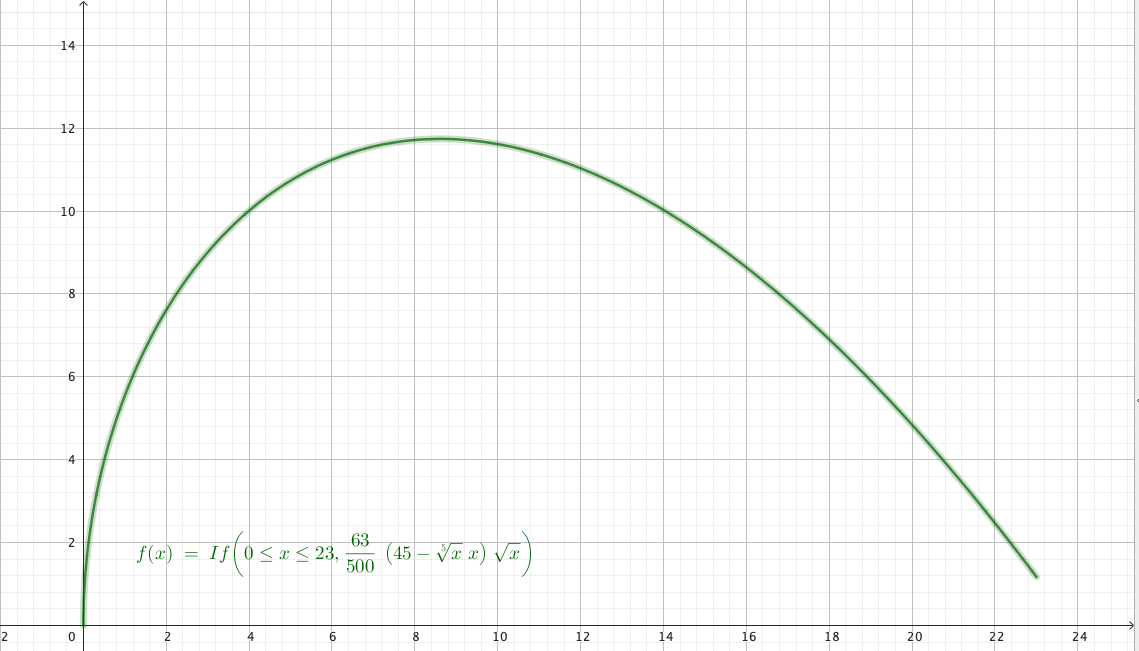
\includegraphics[scale=0.4]{graf.png}
\end{center}
\caption{Grafen for $f$ tegnet i GeoGebra }
\label{fig:graf}
\end{figure}
Vi kan nu beregne bredden af ballonen.
\begin{equation*}
\begin{split}
  b&=2 \cdot f\left(\left(\frac{2,835}{0,2142}\right) ^{\frac{5}{6}}\right) \\
  &\approx 23,5
\end{split}
\end{equation*}
som er regnet med CAS (se \cref{fig:ballon}).
Altså er ballonens bredde $23,5 \;\unit{m} $.
\begin{figure}[H]
\begin{center}
  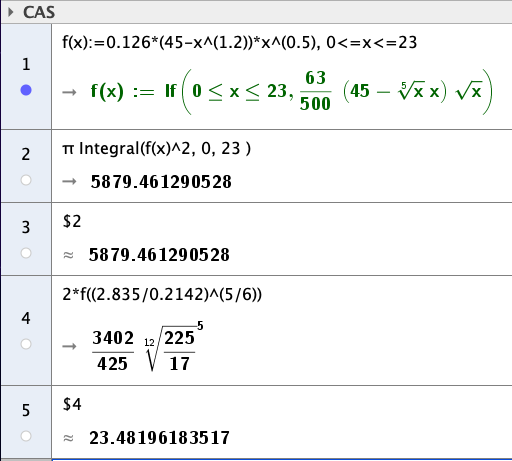
\includegraphics[scale=0.5]{ballon.png}
\end{center}
\caption{Udtrykket for volumen og bredde udregnet med CAS}
\label{fig:ballon}
\end{figure}
\begin{question}{Opgave 11}{}
 En differentialligning er givet ved

$$y'=y+x^2.$$
\begin{itemize}
  \item[a.] Tegn et hældningsfelt for differentialligningen.
\end{itemize}
Det oplyses, at funktionen $f$ er løsning til differentialligningen, og at grafen for $f$ går gennem punktet $P(0,-1).$
\begin{itemize}
  \item[b.] Bestem en forskrift for $f.$ 
\end{itemize}
\end{question}
\sol \\
\textbf{a.}
Hældningsfeltet for differentialligningen ses i \cref{fig:hældningsfelt}.
\begin{figure}[H]
\begin{center}
  \includegraphics[width=\textwidth]{hældningsfelt.png }
\end{center}
\caption{Hældningsfelt for differentialligningen tegnet i GeoGebra}
\label{fig:hældningsfelt}
\end{figure}
\textbf{b.}
Vi finder først den fuldstændige løsning for differentialligningen med panserformlen.
Siden $A(x)=-x$ er en stamfunktion til $a(x)=-1$, så gælder
\begin{equation*}
\begin{split}
  y'=y+x^2 &\iff y'-y=x^2\\
  &\iff y= e^{-(-x)} \int x^2 \cdot e^{-x}  \,dx + c \cdot e^{-(-x)} \\
\end{split}
\end{equation*}
Vi beregner nu integralet med integration med dele (to gange), hvor vi lader $u=x^2$ og $dt=e^{-x}\, dx$, hvilket vil sige, at $du=2x \, dx$ og $t=-e^{-x} $. 
Bemærk at vi ser bort fra konstanten fra integralet.
\begin{equation*}
\begin{split}
  y&=e^{x} \cdot \left(ut- \int t \,du \right) + c \cdot e^{x} \\
  &=e^{x} \cdot \left(-e^{-x} \cdot x^2 - 2\int -e^{-x} x \,dx  \right) + c \cdot e^{x} \\
  &=e^{x} \cdot \left(-e^{-x} \cdot x^2 - 2 \cdot \left(x \cdot e^{-x} - \int e^{-x}  \,dx \right) \right) + c \cdot e^{x} \\
  &=e^{x} \cdot \left(-e^{-x} \cdot x^2 - 2 \cdot \left(x \cdot e^{-x} +e^{-x} \right)  \right) + c \cdot e^{x} \\
  &=e^{x} \cdot e^{-x} \cdot \left(-x^2-2x-2\right) +c \cdot e^{x} \\
  &=-x^2-2x-2 + c \cdot e^{x} 
\end{split}
\end{equation*}
Da grafen for $f$ går gennem $P(0,-1)$, så kan vi finde $c$. 
\begin{equation*}
\begin{split}
  f(0)= -1 &\implies -0^2-2 \cdot 0-2+c \cdot e^{0} =-1\\
  &\iff c-2=-1\\
  &\iff c=1
\end{split}
\end{equation*}
Altså er en forskrift for $f$
\begin{equation*}
\begin{split}
f(x)= -x^2-2x-2 + e^{x} 
\end{split}
\end{equation*}
\begin{question}{Opgave 13}{}
  En isproducent har undersøgt det daglige isforbrug blandt en række forbrugere.
Tabellen viser sammenhørende værdier for det daglige isforbrug og middeltemperaturenden pågældende dag.

I en model kan sammenhængen beskrives ved

$$f(x)=a\cdot x+b,$$

hvor $f(x)$ betegner det daglige isforbrug (målt i liter), og $x$ betegner middeltemperatur målt i $\unit{\celsius} $.
\begin{itemize}
  \item[a.] Benyt regression på tabellens data til at bestemme konstanterne $a$ og $b.$
\end{itemize}
\end{question}
\sol \\
\textbf{a.}
Vi laver en lineær regression i Excel, hvilket ses i \cref{fig:excel}.
\begin{figure}[H]
\begin{center}
  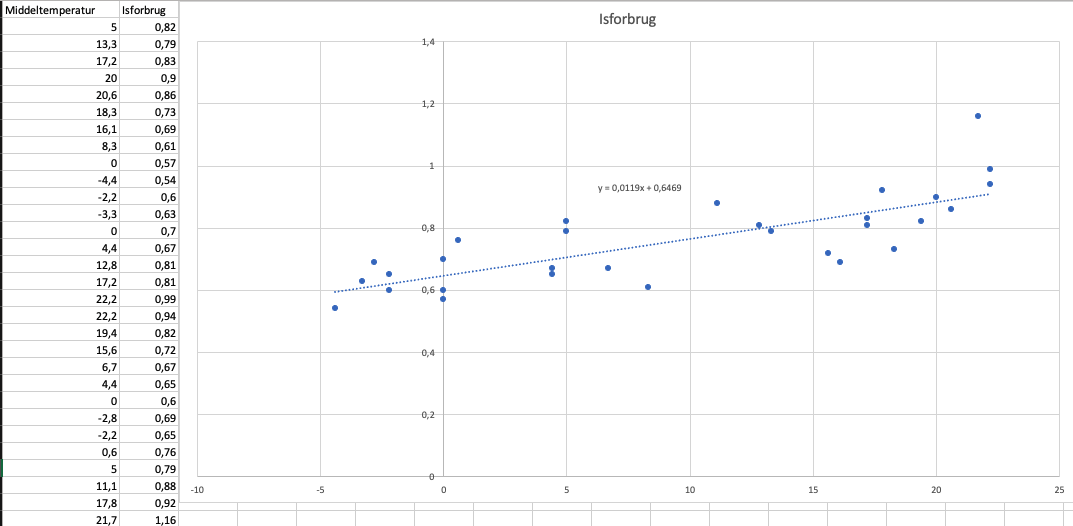
\includegraphics[scale=0.4]{excel.png}
\end{center}
\caption{Regression lavet i Excel}
\label{fig:excel}
\end{figure}
Fra regressionen har vi, at 
\begin{equation*}
\begin{split}
  y=f(x)=0,0119x + 0,6469
\end{split}
\end{equation*}
Altså må konstanterne være 
\begin{equation*}
\begin{split}
  a&=0,0119\\
  b&=0,6469
\end{split}
\end{equation*}
\begin{question}{Opgave 14}{}
  En funktion $f$ af to variable er givet ved
$$f(x,y)=\begin{pmatrix}x-1\end{pmatrix}^2+(y-2)^3+4.$$
\begin{itemize}
  \item[a.] Tegn grafen for $f$ i grafvinduet [0,2]×[0,4]×[0,10].
\end{itemize}
Det oplyses, at grafen for $f$ har et stationært punkt i $P(x_0,y_0,f(x_0,y_0)).$
\begin{itemize}
  \item[b.] Bestem $x_0$ og $y_0.$
\end{itemize}
\end{question}
\sol \\
\textbf{a.}
Grafen for $f$ i grafvinduet [0,2]×[0,4]×[0,10] ses i \cref{fig:tovar}.
\begin{figure}[H]
\begin{center}
  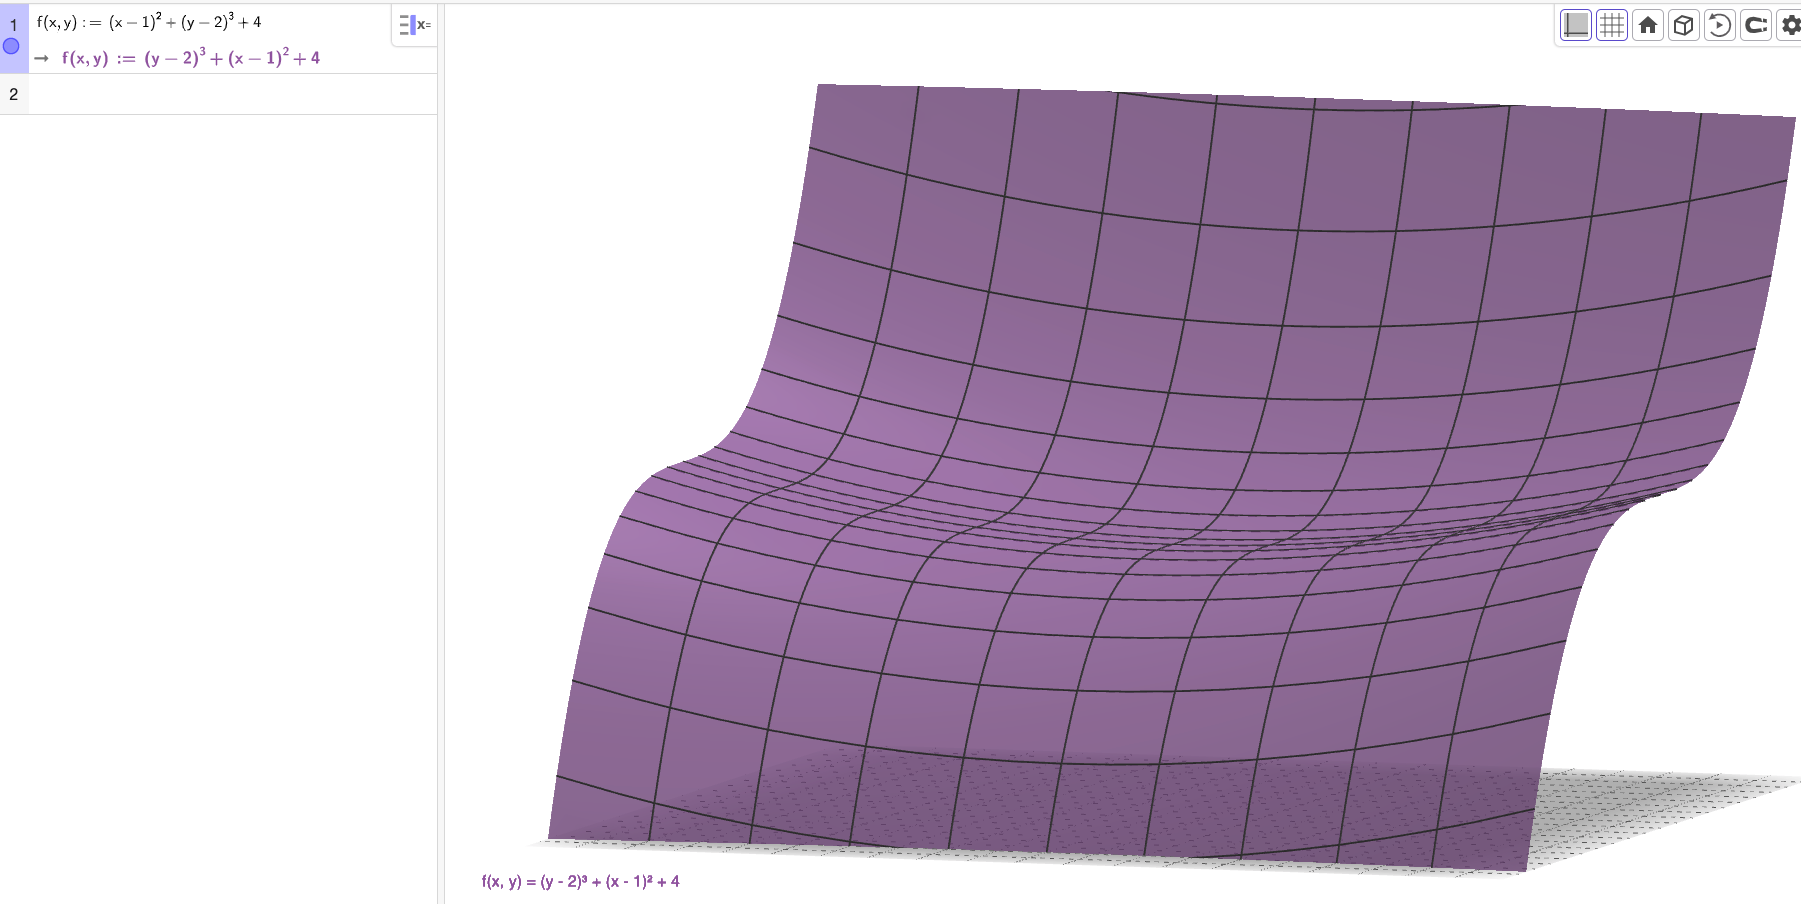
\includegraphics[width=\textwidth]{tovar.png}
\end{center}
\caption{Grafen for $f$ i grafvinduet [0,2]×[0,4]×[0,10] tegnet i GeoGebra}
\label{fig:tovar}
\end{figure}
GeoGebra tegner ikke akserne når man vælger grafvinduet? \\[1ex]
\textbf{b.}
Vi finder først et udtryk for gradienten for $f$.
\begin{equation*}
\begin{split}
  \grad f(x,y)&= \mqty(\pdv{x} \left(\begin{pmatrix}x-1\end{pmatrix}^2+(y-2)^3+4\right) \\ \pdv{y} \left(\begin{pmatrix}x-1\end{pmatrix}^2+(y-2)^3+4\right) ) \\
  &=\mqty(\pdv{x} \left(x^2-2x+1\right) \\ \pdv{y} \left(y^3-6y^2+12y-8\right) ) \\
  &=\mqty(2x-2\\ 3y^2-12y+12) 
\end{split}
\end{equation*}
Siden $P(x_0,y_0,f(x_0,y_0))$ er et stationært punkt for $f$, så må der gælde, at 
\begin{equation*}
\begin{split}
  \grad f(x_0,y_0)= \mqty(0\\ 0) &\iff \mqty(2x_0-2\\ 3y_0^2-12y_0+12) = \mqty(0\\ 0) \\
  &\iff 2x_0=2 \land 3 \cdot \left(y^2-4y+4\right) =0\\
  &\iff x_0=1 \land \left(y-2\right)^2=0\\
  &\iff x_0=1 \land y_0=2
\end{split}
\end{equation*}
Vi har altså bestemt $x_0=1$ og $y_0=2$. 
\begin{question}{Opgave 15}{}
  En krage flyver hen over en sti og taber en nød. I en model kan nøddens position i et koordinatsystem med enheden meter på begge akser beskrives ved

$$\vec{s}(t)=\begin{pmatrix}x(t)\\y(t)\end{pmatrix}=\begin{pmatrix}5t\\30-4,91\cdot t^2\end{pmatrix},\:t\ge0\:,$$

hvor $\vec{s}(t)$ betegner stedvektoren til nøddens position over stien til tidspunktet $t$ (målt i sekunder).
\begin{itemize}
  \item[a.] Benyt modellen til at bestemme nøddens fart $\left|\vec{s}^{\prime}(t)\right|$ til tidspunktet $t=1.$
\end{itemize}
Det oplyses, at længden af en parameterkurve med koordinatfunktioner $x$ og $y$ samt parameteren $t$ i intervallet $[t_1,t_2]$ kan beregnes ved formlen
$$\int_{t_1}^{t_2}\sqrt{\left(x'(t)\right)^2+\left(y'(t)\right)^2}\:dt.$$
\begin{itemize}
  \item[b.] Benyt modellen til at bestemme længden af den banekurve nødden følger, inden den rammer stien.
\end{itemize}
\end{question}
Vi finder først et udtryk for den afledede funktion for $\va{s} $.
\begin{equation*}
\begin{split}
  \va{s}'(t)&=\mqty(\dv{t} \left(5t\right) \\ \dv{t} \left(30-4,91 \cdot t^2\right) ) \\
  &=\mqty(5\\ -9,82 \cdot t) 
\end{split}
\end{equation*}
Vi beregner nu nøddens fart til tidspunktet $t=1$.
\begin{equation*}
\begin{split}
  \abs{\va{s}'(1)} &=\abs{\mqty(5\\ -9,82 \cdot 1) } \\
  &=\sqrt{5^2+\left(-9,82\right)^2} \\
  &\approx 11,02
\end{split}
\end{equation*}
Nøddens fart til tidspunktet $t=1$ er altså $11,02 \;\unit{m/s} $.\\[1ex]
\textbf{b.}
Vi finder først værdien af $t$ når nødden rammer jorden, hvor $y(t)=0$. 
\begin{equation*}
\begin{split}
  y(t)=0 &\iff 30-4,91 \cdot t^2=0 \\
  &\iff t=\sqrt{\frac{30}{4,91}} 
\end{split}
\end{equation*}
da $t$ er positiv. 

\noindent Vi kan nu beregne længden af banekurven, som nødden følger, inden den rammer stien (bemærk at $\abs{\va{s}'(t)} =\sqrt{\left(x'(t)\right)^2 + \left(y'(t)\right)^2} $).
\begin{equation*}
\begin{split}
  \int_{0}^{\sqrt{\frac{30}{4,91}} } \sqrt{5^2 + \left(-9,82 \cdot t\right)^2}  \,dt &=\frac{5 \; \sqrt{9047166} - 625 \; \ln\left(-1250 \; \sqrt{14730} + 1250 \; \sqrt{15355} \right) + 1250 \; \ln\left(125 \right) + 625 \; \ln\left(2 \right)}{491}
  &\approx 33,54
\end{split}
\end{equation*}
som er regnet med CAS (se \cref{fig:CAS}).
Længden af den banekurve nødden følger, inden den rammer stien er altså $33,54 \;\unit{m} $.

\begin{figure}[H]
\begin{center}
  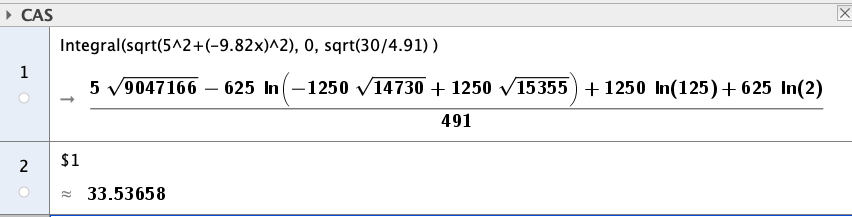
\includegraphics[scale=0.5]{CAS.png}
\end{center}
\caption{Længden af banekuven regnet med CAS}
\label{fig:CAS}
\end{figure}

\end{document}
